\subsection{Error evaluation with exact solution}
\quad We study a numerical experiment with the exact solution of heat equation and evaluate the error convergence. Consider a square $\Omega = [0,1]^2$. Find $u(x, t)$ satisfying
\begin{equation}
	\dfrac{\partial u}{\partial t} - \left(\dfrac{\partial^2 u}{\partial x_1^2} + \dfrac{\partial^2u}{\partial x_2^2}\right) = (1+2\pi^2)e^t\sin(\pi x_1) \sin(\pi x_2),
\end{equation}
with the initial and boundary conditions
$$ u(x, 0) = \sin(\pi x_1)\sin(\pi x_2) \quad \text{and} \quad u|_S = 0.$$
The exact solution is
$$u(x, t) = e^t\sin(\pi x_1) \sin(\pi x_2), $$

In order to quantify the difference between the approximate solution and the exact one, different cases of mesh size and time step length were studied to show the convergence of $L^2$-error. Fig. \ref{fig:time} shows, for this error measurement, the convergence of the approximate solution to the exact one when the time step tends to zero. Remark that, for each $h$, the error tends to a constant that is independent of time step. Numerically, we are looking for a representation of the error as the sum of two terms, one depends on $h$ and the other depend on $\Delta t$: $\left\|u_h-u\right\|_{L^2(Q)}=O\left(h^{\alpha}+\Delta t^{p}\right)$. Fig \ref{fig:mesh} shows the error versus $h$ for various mesh size, the time step $\Delta t$ has been chosen sufficiently small such that the error depends only upon $h$. Observe that the approximate solution converges to the exact one with mesh refinement with a power index $\alpha \approx 2$. This result is in good accordance with the Theorem \ref{dl2.1} in the previous section.
\begin{figure}[h!]
	\centering
	\begin{tabular}{c}
		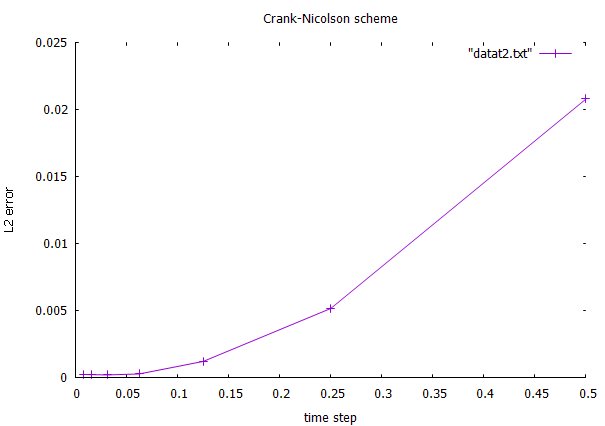
\includegraphics[width=.8\linewidth]{figures/CNt}
	\end{tabular}
	\caption{$L^2$ error convergence of Crank-Nicolson scheme depends on time step.}
	\label{fig:time}
\end{figure}
\begin{figure}[h!]
	\centering
	\begin{tabular}{c}
		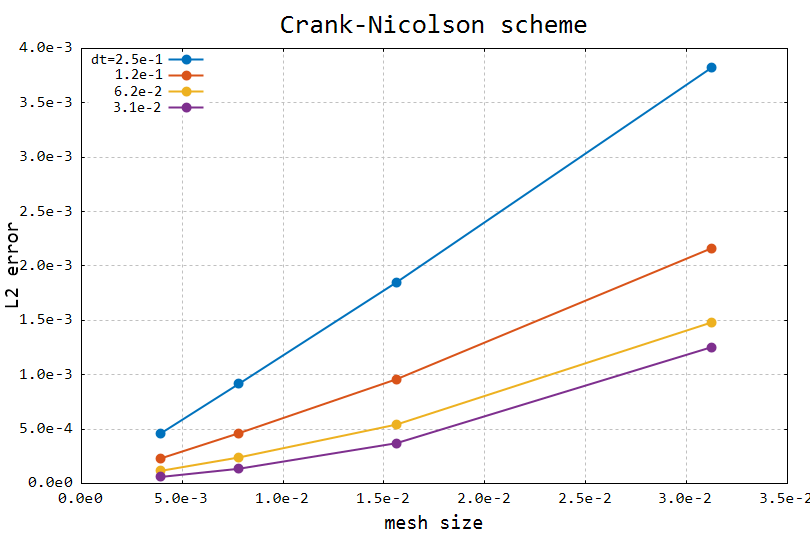
\includegraphics[width=.8\linewidth]{figures/CN}
	\end{tabular}
	\caption{$L^2$ error convergence of Crank-Nicolson scheme depends on mesh size.}
	\label{fig:mesh}
\end{figure}

\subsection{A problem of thermal engineering}
\quad The parameters $a_{ji}$ in \eqref{1.1} describe thermal conductivity property of a specific object. For a homogeneity object, thermal conductions are equal for all dimensions, which mean $a_{ji}=const \quad \forall i,j=\overline{1,d}$. The constant is thermal conductivity coefficient of the object material. In two dimensional case, \eqref{1.1} forms as
\begin{align}\label{4.2}
	\dfrac{\partial u}{\partial t} - \kappa \left(\dfrac{\partial^2 u}{\partial x_1^2}+\dfrac{\partial^2 u}{\partial x_2^2}\right) = F.
\end{align}
\quad We apply the numerical simulations of heat transfer into designing heat sink. Assuming a hot CPU inside a rectangular room fill with air. Let $u=u_{hot}$ inside CPU region and $u=u_{air}$ on air region, respectively $\Omega_{c}$ and $\Omega_{a}$, on the initial time. Our goal is to design a heat sink stick on the CPU to lower its temperature. Figure \ref{fig:testsink} describes the setting of this experiment.\\
\begin{figure}[ht]
	\centering
	\begin{tikzpicture}
		\draw (0,0) -- (6,0);
		\draw (6,0) -- (6,4);
		\draw (6,4) -- (0,4);
		\draw (0,4) -- (0,0);
		\draw (4,0) -- (4,0.8);
		\draw (4,0.8) -- (2,0.8);
		\draw (2,0.8) -- (2,0);
		\node at (3,0.4) {$\Omega_c$};
		\node at (3,2.5) {$\Omega_a$};
		\node at (3,1.1) {$\Omega_s$};
		\draw (2,1.5) .. controls (2.7,2) and (3.4,1) .. (4,1.2);
		\draw (2,0.8) -- (2,1.5);
		\draw (4,0.8) -- (4,1.2);
	\end{tikzpicture}
	\caption{Illustration of simple cooling system for CPU.}
	\label{fig:testsink}
\end{figure}
\newpage
The heat sink region, denoted by $\Omega_{s}$, has thermal conductivity coefficient $\kappa_s$. Similarly, let $\kappa_a$ and $\kappa_c$ be respectively the thermal conductivity coefficients inside air and CPU region. Technically, $\kappa_a$ value is small compared to $\kappa_c$ and $\kappa_s$ due to thermal conducting nature of air. Furthermore, to provide cooling ability, $\kappa_s>\kappa_c$. The visualization using medit software. At initial state, set $u_{hot}=80$ and $u_{air}=20$ as in Figure \ref{fig:ini}.\\
\begin{figure}[http]
	\centering
	\begin{tabular}{c}
		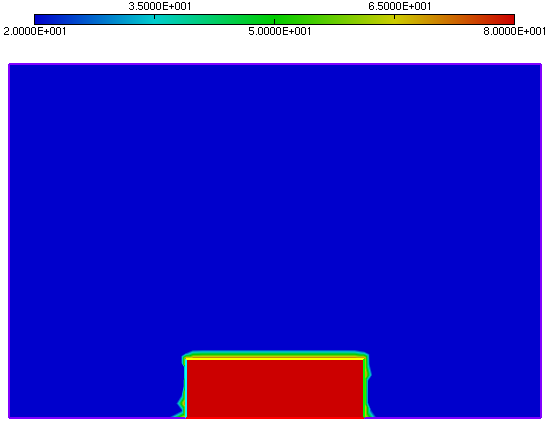
\includegraphics[width=.8\linewidth]{figures/begin}
	\end{tabular}
	\caption{Thermal distribution at initial state. $u|_{\Omega_{c}} = 80$, $u|_{\Omega_{a}\cup\Omega_{s}}=20$.}
	\label{fig:ini}
\end{figure}\\
Set $T=1s$, $\kappa_a=0.01$, $\kappa_c=1$, $\kappa_s=100$. The thermal distribution, maximum and minimum temperature inside domain $\Omega_{c}$  at final time $T$ of different heat sink shapes are shown in Figures \ref{fig:nosink}, \ref{fig:recsink} and \ref{fig:finsink}.\\
\begin{figure}[http]
	\centering
	\begin{tabular}{c}
		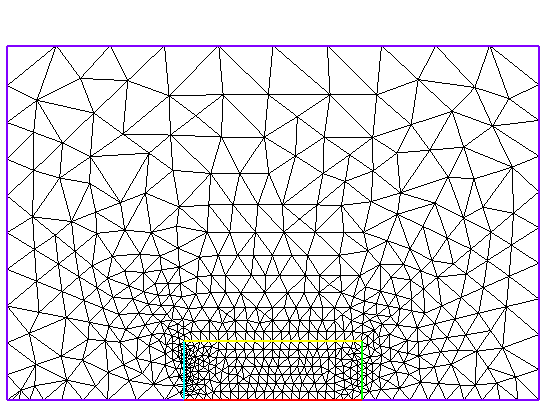
\includegraphics[width=.8\linewidth]{figures/nosinkc} \\ 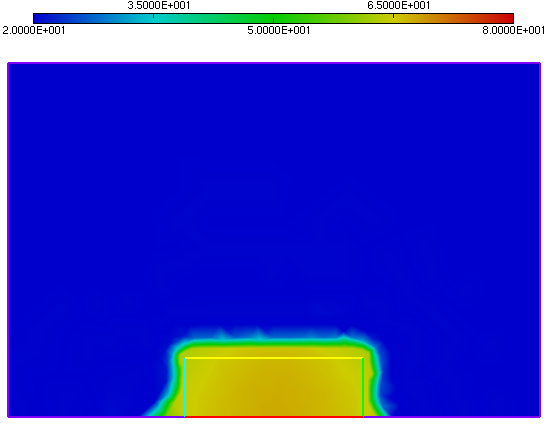
\includegraphics[width=.8\linewidth]{figures/nosinkb}
	\end{tabular}
	\caption{Thermal conduction without heat sink. $u_{min}=63.1$, $u_{max}=67.3$.}
	\label{fig:nosink}
\end{figure}
\begin{figure}[http]
	\centering
	\begin{tabular}{c}
		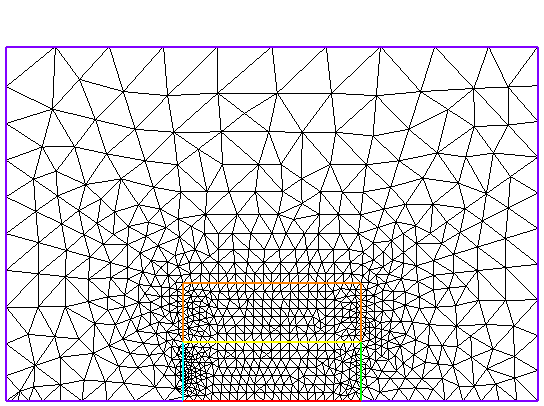
\includegraphics[width=.8\linewidth]{figures/recsinkc} \\ 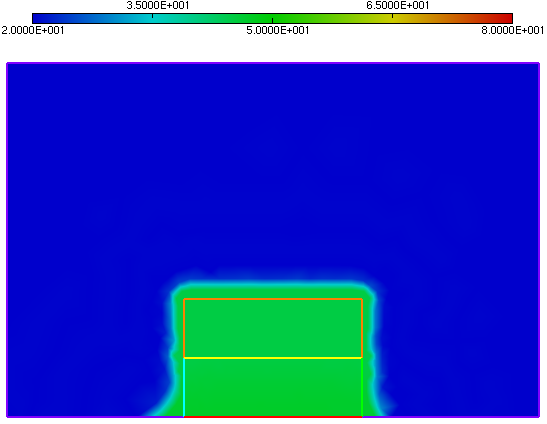
\includegraphics[width=.8\linewidth]{figures/recsinkb}
	\end{tabular}
	\caption{Thermal conduction with rectangular shape heat sink. $u_{min}=44.8$, $u_{max}=46.9$.}
	\label{fig:recsink}
\end{figure}
\begin{figure}[ht]
	\centering
	\begin{tabular}{c}
		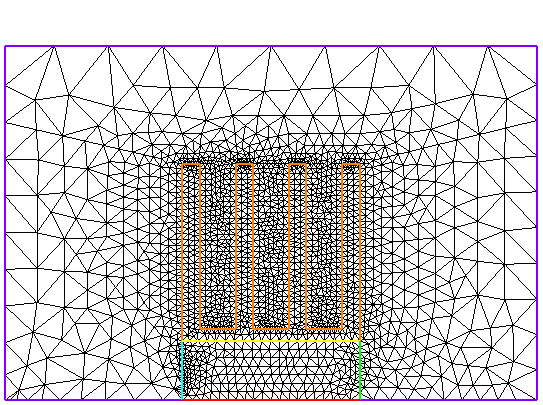
\includegraphics[width=.8\linewidth]{figures/finsinkc} \\ 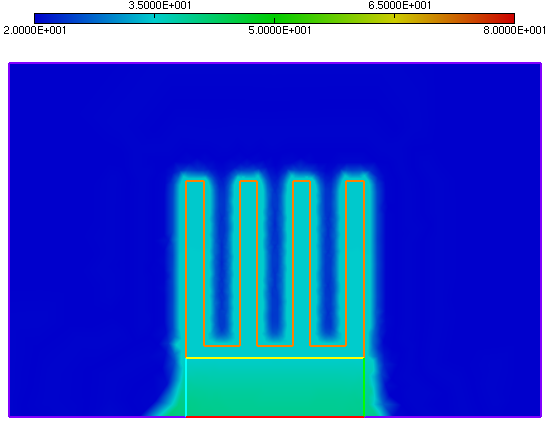
\includegraphics[width=.8\linewidth]{figures/finsinkb}
	\end{tabular}
	\caption{Thermal conduction with fin shape heat sink. $u_{min}=34.9$, $u_{max}=40.1$.}
	\label{fig:finsink}
\end{figure}
